%%%%%%%%%%%%%%%%%%%%%%%%%%%%%%%%%%%%%%%%%
% University Assignment Title Page 
% LaTeX Template
%
% This template has been downloaded from:
% http://www.latextemplates.com
%
% Original author:
% WikiBooks (http://en.wikibooks.org/wiki/LaTeX/Title_Creation)
% 
% Instructions for using this template:
% This title page is presently capable of being compiled as is. This is not 
% useful for including it in another document. To do this, you have two options: 
%
% 1) Copy/paste everything between \begin{document} and \end{document} 
% starting at \begin{titlepage} and paste this into another LaTeX file where you 
% want your title page.
% OR
% 2) Remove everything outside the \begin{titlepage} and \end{titlepage} and 
% move this file to the same directory as the LaTeX file you wish to add it to. 
% Then add \input{./title_page_1.tex} to your LaTeX file where you want your
% title page.
%
%%%%%%%%%%%%%%%%%%%%%%%%%%%%%%%%%%%%%%%%%

%----------------------------------------------------------------------------------------
%	PACKAGES AND OTHER DOCUMENT CONFIGURATIONS
%----------------------------------------------------------------------------------------

\begin{titlepage}

\newcommand{\HRule}{\rule{\linewidth}{0.5mm}} % Defines a new command for the horizontal lines, change thickness here

\center % Center everything on the page
 
%----------------------------------------------------------------------------------------
%	HEADING SECTIONS
%----------------------------------------------------------------------------------------

\textsc{\LARGE Université Pierre et Marie Curie}\\[1.5cm] % Name of your university/college
\textsc{\Large \titletype}\\[0.5cm] % Major heading such as course name
\textsc{\large PIAD de Master1 d’Informatique en Intelligence Artificielle et Décision}\\[0.5cm] % Minor heading such as course title

%----------------------------------------------------------------------------------------
%	TITLE SECTION
%----------------------------------------------------------------------------------------

\HRule \\[0.4cm]
{ \huge \bfseries Semi-supervised Learning Agents}\\[0.4cm] % Title of your document
\HRule \\[1.5cm]
 
 
%
\includegraphics[height=60mm]{images/torcs.png}\\[1cm]
 
 
%----------------------------------------------------------------------------------------
%	AUTHOR SECTION
%----------------------------------------------------------------------------------------

\begin{minipage}{0.4\textwidth}
\begin{flushleft} \large
\emph{Auteurs:}\\
Lan \textsc{Zhou}\\ % Your name
Matthieu \textsc{Zimmer} % Your name
\end{flushleft}
\end{minipage}
~
\begin{minipage}{0.4\textwidth}
\begin{flushright} \large
\emph{Superviseurs:} \\
Paolo \textsc{Viappiani}\\ % Supervisor's Name
Paul \textsc{Weng}\\ % Supervisor's Name
\end{flushright}
\end{minipage}\\[1cm]

\vfill

%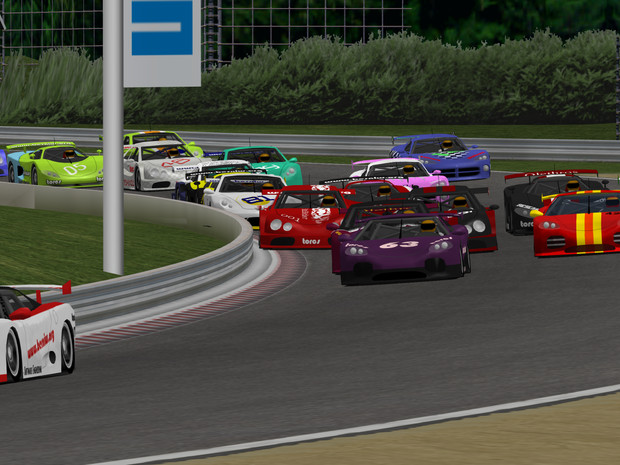
\includegraphics[height=70mm]{images/torcs.jpg}\\[1cm]

%----------------------------------------------------------------------------------------
%	DATE SECTION
%----------------------------------------------------------------------------------------

{\large \today}\\[3mm] % Date, change the \today to a set date if you want to be precise
{\large Version 1.1}\\[1.5cm] 

%----------------------------------------------------------------------------------------
%	LOGO SECTION
%----------------------------------------------------------------------------------------


\includegraphics[height=13mm]{../images/logo.png} % Include a department/university logo - this will require the graphicx package

%----------------------------------------------------------------------------------------

% \vfill % Fill the rest of the page with whitespace

\end{titlepage}